\documentclass[handout]{beamer}
\usetheme{metropolis}
\beamertemplatetransparentcoveredhigh

\usepackage[portuges]{babel}
\usepackage{graphicx}
\graphicspath{{./figs/}}
\usepackage{listings}
\usepackage{color}
\usepackage{hyperref}
\usepackage{xpatch}
\usepackage{comment}
\usepackage[outputdir=build]{minted}

\makeatletter
\AtBeginEnvironment{minted}{\dontdofcolorbox}
\def\dontdofcolorbox{\renewcommand\fcolorbox[4][]{##4}}
\xpatchcmd{\inputminted}{\minted@fvset}{\minted@fvset\dontdofcolorbox}{}{}
\xpatchcmd{\mintinline}{\minted@fvset}{\minted@fvset\dontdofcolorbox}{}{}
\makeatother
\setminted[c]{
  linenos=true,
  breaklines=true,
  encoding=utf8,
  frame=lines,
  framerule=0.5pt,
  autogobble,
  fontsize=\small,
}
\setminted[bash]{
  linenos=true,
  encoding=utf8,
  frame=lines,
  framerule=0.5pt,
  autogobble,
  fontsize=\small
}

\newcommand{\cod}[1]{\mintinline{c}{#1}}


\definecolor{dkgreen}{rgb}{0,0.6,0}
\definecolor{gray}{rgb}{0.5,0.5,0.5}
\definecolor{mauve}{rgb}{0.58,0,0.82}


\definecolor{Purple}{HTML}{911146}
\definecolor{Orange}{HTML}{CF4A30}
\setbeamercolor{alerted text}{fg=Orange}
\setbeamercolor{frametitle}{bg=Purple}
\setbeamercolor{block body}{bg=Purple!20,fg=black}
\setbeamercolor{block title}{bg=Purple!50,fg=black}
\setbeamertemplate{blocks}[rounded][shadow=true]


\newcounter{ExercicioCounter}
\newcommand{\exercicio}{\refstepcounter{ExercicioCounter} Exercício~\theExercicioCounter}

\newcommand{\setcoverbg}{
  \setbeamertemplate{background}
  {
\includegraphics[width=\paperwidth,height=\paperheight]{backgrounds/coverbg}}
}
\newcommand{\setsectionbg}{
  \setbeamertemplate{background}
  {
\includegraphics[width=\paperwidth,height=\paperheight]{backgrounds/blank}}
}

\title{Programação Estruturada}
\subtitle{Ponteiros --- Parte 1}

\author{Professores Emílio Francesquini e Carla Negri Lintzmayer}
\institute{Centro de Matemática, Computação e Cognição\\ Universidade Federal do ABC}
\date{2018.Q3}

\begin{document}

\setcoverbg
\maketitle
\setsectionbg


%\begin{frame}{Roteiro}
%    \tableofcontents
%\end{frame}


%%%%%%%%%%%%%%%%%%%%%%%%%%%%%%%%%%%%%%%%%%
%%%%%%%%%%%%%%%%%%%%%%%%%%%%%%%%%%%%%%%%%%
%%%%%%%%%%%%%%%%%%%%%%%%%%%%%%%%%%%%%%%%%%
%%%%%%%%%%%%%%%%%%%%%%%%%%%%%%%%%%%%%%%%%%
%%%%%%%%%%%%%%%%%%%%%%%%%%%%%%%%%%%%%%%%%%
%%%%%%%%%%%%%%%%%%%%%%%%%%%%%%%%%%%%%%%%%%


\section{Ponteiros}

%%%%%%%%%%%%%%%%%%%%%%%%%%%%%%%%%%%%%%%%%%
\begin{frame}[fragile]{Ponteiro}

    \begin{itemize}[<+->]
        \item Ponteiros são tipos especiais de dados que armazenam endereços de memória.
        \item Uma variável do tipo ponteiro deve ser declarada da seguinte forma:
        \begin{minted}{c}
            tipo *nome_variável;
        \end{minted}
        \item A variável ponteiro armazenará um endereço de memória de uma outra variável do tipo especificado.
        \item Exemplo:
        \begin{minted}{c}
            int *mema; float *memb;
        \end{minted}
        {\bf mema} armazena um endereço de memória de variáveis do tipo {\bf int}.\\
        {\bf memb} armazena um endereço de memória de variáveis do tipo {\bf float}.\\
    \end{itemize}

\end{frame}

%%%%%%%%%%%%%%%%%%%%%%%%%%%%%%%%%%%%%%%%%%
%%%%%%%%%%%%%%%%%%%%%%%%%%%%%%%%%%%%%%%%%%
%%%%%%%%%%%%%%%%%%%%%%%%%%%%%%%%%%%%%%%%%%
%%%%%%%%%%%%%%%%%%%%%%%%%%%%%%%%%%%%%%%%%%
%%%%%%%%%%%%%%%%%%%%%%%%%%%%%%%%%%%%%%%%%%


\subsection{Operadores de Ponteiros}

%%%%%%%%%%%%%%%%%%%%%%%%%%%%%%%%%%%%%%%%%%
\begin{frame}[fragile]{Operadores de Ponteiro}
    \begin{itemize}[<+->]
        \item Existem dois operadores relacionados aos ponteiros:
        \begin{itemize}
            \item O operador {\bf \&} retorna o endereço de memória de uma variável:
            \begin{minted}{c}
                int *mema;
                int a = 90;
                mema = &a;
            \end{minted}
            \item O operador {\bf *} acessa o conteúdo do endereço indicado pelo ponteiro:
            \begin{minted}{c}
                printf("%d", *mema);
            \end{minted}
        \end{itemize}
    \end{itemize}
    \pause
    \begin{center}
        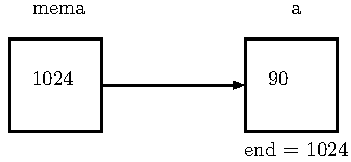
\includegraphics[width=5cm]{ponteiro.pdf}
    \end{center}
\end{frame}

%%%%%%%%%%%%%%%%%%%%%%%%%%%%%%%%%%%%%%%%%%
\begin{frame}[fragile]{Operadores de Ponteiro}
    \begin{small}
        \begin{minted}{c}
            #include <stdio.h>

            int main() {
                int b;
                int *c;

                b = 10;
                c = &b;
                *c = 11;
                printf("%d\n", b);
                return 0;
            }
        \end{minted}
    \end{small}
    \textbf{O que será impresso?}
\end{frame}


%%%%%%%%%%%%%%%%%%%%%%%%%%%%%%%%%%%%%%%%%%
\begin{frame}[fragile]{Operadores de Ponteiro}
    \begin{small}
        \begin{minted}{c}
            #include <stdio.h>

            int main() {
                int num, q = 1;
                int *p;

                num = 100;
                p = &num;
                q = *p;

                printf("%d\n", q);
                return 0;
            }
        \end{minted}
    \end{small}
    \textbf{O que será impresso?}

\end{frame}



%%%%%%%%%%%%%%%%%%%%%%%%%%%%%%%%%%%%%%%%%%
\begin{frame}[fragile]{Cuidado 1!}
    \begin{itemize}[<+->]
        \item Não se pode atribuir um valor para o endereço apontado
        pelo ponteiro sem antes ter certeza de que o endereço é válido:
        \begin{minted}{c}
            int a, b;
            int *c;

            b = 10;
            *c = 13; /* Vai armazenar 13 em qual endereço? */
        \end{minted}
        \item O correto seria por exemplo:
        \begin{minted}{c}
            int a, b;
            int *c;

            b = 10;
            c = &a;
            *c = 13;
        \end{minted}
    \end{itemize}
\end{frame}

\begin{frame}[fragile]{Cuidado 2!}
    \begin{itemize}
        \item Infelizmente o operador {\bf *} de ponteiros é igual ao da multiplicação.
        Portanto preste atenção em como utilizá-lo.
        \begin{minted}[fontsize=\footnotesize]{c}
            #include <stdio.h>

            int main() {
                int b, a;
                int *c;
                b = 10;
                c = &a;
                *c = 11;
                a = b * c;
                printf("%d\n", a);
                return 0;
            }
        \end{minted}

        \item Ocorre um erro de compilação pois o {\bf *} é interpretado como operador de
        ponteiro sobre {\bf c} e não de multiplicação.
    \end{itemize}
\end{frame}



\begin{frame}[fragile]{Cuidado 2!}
    \begin{itemize}
        \item O correto seria algo como:
        \begin{minted}{c}
            #include <stdio.h>

            int main() {
                int b, a;
                int *c;

                b = 10;
                c = &a;
                *c = 11;
                a = b * (*c);
                printf("%d\n", a);
                return 0;
            }
        \end{minted}
    \end{itemize}
\end{frame}


%%%%%%%%%%%%%%%%%%%%%%%%%%%%%%%%%%%%%%%%%%
\begin{frame}[fragile]{Cuidado 3!}
    \begin{itemize}
        \item O endereço que um ponteiro armazena é sempre de um tipo específico.
        \begin{minted}[fontsize=\footnotesize]{c}
            #include <stdio.h>

            int main() {
                double b, a;
                int *c;
                b = 10.89;
                c = &b; /* Ops! c é ponteiro para int e não double */
                a = *c;
                printf("%lf\n", a);
                return 0;
            }
        \end{minted}
        \item Além do compilador alertar que a atribuição pode causar problemas, é impresso
        um valor totalmente diferente de $10.89$.
    \end{itemize}
\end{frame}

%%%%%%%%%%%%%%%%%%%%%%%%%%%%%%%%%%%%%%%%%%
\begin{frame}[fragile]{Operações com ponteiros}

    Podemos comparar ponteiros ou o conteúdo apontado por eles:
    \begin{minted}[fontsize=\scriptsize]{c}
        int main() {
            double *a, *b, c, d;
            b = &c;
            a = &d;

            if (b < a)
                printf("O endereco apontado por b eh menor: %p e %p\n", b, a);
            else if (a < b)
                printf("O endereco apontado por a eh menor: %p e %p\n", a, b);
            else if (a == b)
                printf("Mesmo endereco");

            if (*a == *b)
                printf("Mesmo conteudo: %lf\n", *a);
            return 0;
        }
    \end{minted}

    {\bf Notem que para imprimir um ponteiro usamos \%p}.
\end{frame}

%%%%%%%%%%%%%%%%%%%%%%%%%%%%%%%%%%%%%%%%%%
%%%%%%%%%%%%%%%%%%%%%%%%%%%%%%%%%%%%%%%%%%
%%%%%%%%%%%%%%%%%%%%%%%%%%%%%%%%%%%%%%%%%%
%%%%%%%%%%%%%%%%%%%%%%%%%%%%%%%%%%%%%%%%%%
%%%%%%%%%%%%%%%%%%%%%%%%%%%%%%%%%%%%%%%%%%


\subsection{O valor NULL}


%%%%%%%%%%%%%%%%%%%%%%%%%%%%%%%%%%%%%%%%%%
\begin{frame}[fragile]{O valor NULL}

    \begin{itemize}
        \item Quando um ponteiro não está associado com nenhum endereço válido
        é comum atribuir o valor {\bf NULL} para este.
        \item Isto é usado em comparações com ponteiros para saber se um determinado
        ponteiro possui valor válido ou não.
        \item O que é impresso se fizermos: \mintinline{c}{printf("%p\n", NULL);} ?
    \end{itemize}

    \begin{minted}{c}
        int main() {
            double *a = NULL, *b = NULL, c = 5;
            a = &c;
            if (a != NULL) {
                b = a;
                printf("Numero: %lf\n", *b);
            }
            return 0;
        }
    \end{minted}

\end{frame}


%%
%%%%%%%%%%%%%%%%%%%%%%%%%%%%%%%%%%%%%%%%
%%%%%%%%%%%%%%%%%%%%%%%%%%%%%%%%%%%%%%%%%%
%%%%%%%%%%%%%%%%%%%%%%%%%%%%%%%%%%%%%%%%%%
%%%%%%%%%%%%%%%%%%%%%%%%%%%%%%%%%%%%%%%%%%
%%%%%%%%%%%%%%%%%%%%%%%%%%%%%%%%%%%%%%%%%%
%%%%%%%%%%%%%%%%%%%%%%%%%%%%%%%%%%%%%%%%%%
%%%%%%%%%%%%%%%%%%%%%%%%%%%%%%%%%%%%%%%%%%
%%%%%%%%%%%%%%%%%%%%%%%%%%%%%%%%%%%%%%%%%%
%%%%%%%%%%%%%%%%%%%%%%%%%%%%%%%%%%%%%%%%%%

\section{Passagem de Parâmetros por Valor e por Referência}

%%%%%%%%%%%%%%%%%%%%%%%%%%%%%%%%%%%%%%%%%%%%%%

\begin{frame}[fragile]{Passagem de parâmetros}

    \small
    \begin{itemize}[<+->]
        \item Quando passamos argumentos para uma função, os valores fornecidos
        são copiados para as variáveis parâmetros da função. Este processo é
        idêntico a uma atribuição. {\bf Este processo é chamado de passagem por valor.}
        \item Desta forma, alterações nos parâmetros dentro da função não
        alteram os valores que foram passados na chamada da função:
        \vspace{-1em}
        \begin{minted}[fontsize=\footnotesize]{c}
            int main() {
                int a = 4, b = 5;
                nao_troca(a, b);
                return 0;
            }
            void nao_troca(int x, int y) {
                int aux;
                aux = x;
                x = y;
                y = aux;
            }
        \end{minted}
    \end{itemize}

\end{frame}

%%%%%%%%%%%%%%%%%%%%%%%%%%%%%%%%%%%%%%%%%%%%%%

\begin{frame}[fragile]{Passagem de argumentos por referência}

    \begin{itemize}
        \item Em C só existe passagem de parâmetros por valor.
        \item Em algumas linguagens existem construções para se {\bf passar parâmetros
          por referência}.
        \begin{itemize}
            \item Neste último caso, alterações de um parâmetro passado por referência
            também ocorrem onde foi feita a chamada da função.

            \item No exemplo anterior, se x e y fossem passados por referência, seus
            conteúdos seriam trocados.
        \end{itemize}
    \end{itemize}
\end{frame}

%%%%%%%%%%%%%%%%%%%%%%%%%%%%%%%%%%%%%%%%%%%%%%
\begin{frame}[fragile]{Passagem de argumentos por referência}

    \small
    Podemos obter algo semelhante em C utilizando ponteiros.
    \begin{itemize}[<+->]
        \item O artifício corresponde em passar como argumento para uma função
        o \alert{endereço} da variável, e não o seu valor.
        \item Desta forma podemos alterar o conteúdo da variável como se
        fizéssemos passagem por referência.
        \vspace{-1em}
        \begin{minted}[fontsize=\scriptsize]{c}
            #include <stdio.h>
            void troca(int *a, int *b);
            int main() {
                int x = 4, y = 5;
                troca(&x, &y);
                printf("x = %d e y = %d\n", x, y);
                return 0;
            }
            void troca(int *a, int *b) {
                int aux;
                aux = *a;
                *a  = *b;
                *b = aux;
            }
        \end{minted}
    \end{itemize}

\end{frame}


%%%%%%%%%%%%%%%%%%%%%%%%%%%%%%%%%%%%%%%%%%%%%%
\begin{frame}[fragile]{Passagem de argumentos por referência}

    \begin{itemize}[<+->]
        \item O uso de ponteiros para passar parâmetros que devem ser alterados dentro de uma
        função é útil em certas situações como:
        \begin{itemize}
            \item Funções que precisam retornar mais do que um valor.
        \end{itemize}
        \item Suponha que queremos criar uma função que recebe um vetor como parâmetro e precisa retornar
        o maior e o menor elemento do vetor.
        \begin{itemize}
            \item Mas uma função só retorna um único valor!
            \item Podemos passar ponteiros para variáveis que ``receberão'' o maior e menor elemento.
        \end{itemize}

    \end{itemize}

\end{frame}


%%%%%%%%%%%%%%%%%%%%%%%%%%%%%%%%%%%%%%%%%%%%%%
\begin{frame}[fragile]{Passagem de argumentos por referência}
    \begin{minted}[fontsize=\scriptsize]{c}
         #include <stdio.h>
         void maxAndMin(int vet[], int tam, int *min, int *max);
         int main() {
             int v[] = {10, 80, 5, -10, 45, -20, 100, 200, 10};
             int min, max;
             maxAndMin(v, 9, &min, &max);
             printf("O menor eh: %d\nO maior eh: %d\n", min, max);
             return 0;
         }
         void maxAndMin(int vet[], int tam, int *min, int *max) {
             int i;
             *max = vet[0];
             *min = vet[0];
             for (i = 0; i < tam; i++) {
                 if (vet[i] < *min)
                     *min = vet[i];
                 if (vet[i] > *max)
                     *max = vet[i];
             }
         }
    \end{minted}
\end{frame}

%%%%%%%%%%%%%%%%%%%%%%%%%%%%%%%%%%%%%%%%%%%%%%

\begin{frame}[fragile]{Explicando o \cod{scanf}}

    Finalmente sabemos o porquê do \textbf{\&} no \cod{scanf}:

    \begin{minted}{c}
         #include <stdio.h>

         int main() {
             int x;
             int *p;

             scanf("%d", &x);
             scanf("%d", &p); /* ERRO! */

             p = &x;
             scanf("%d", p);
             return 0;
         }
    \end{minted}
\end{frame}


%%%%%%%%%%%%%%%%%%%%%%%%%%%%%%%%%%%%%%%%%%
%%%%%%%%%%%%%%%%%%%%%%%%%%%%%%%%%%%%%%%%%%
%%%%%%%%%%%%%%%%%%%%%%%%%%%%%%%%%%%%%%%%%%
%%%%%%%%%%%%%%%%%%%%%%%%%%%%%%%%%%%%%%%%%%
%%%%%%%%%%%%%%%%%%%%%%%%%%%%%%%%%%%%%%%%%%
%%%%%%%%%%%%%%%%%%%%%%%%%%%%%%%%%%%%%%%%%%
%%%%%%%%%%%%%%%%%%%%%%%%%%%%%%%%%%%%%%%%%%
%%%%%%%%%%%%%%%%%%%%%%%%%%%%%%%%%%%%%%%%%%
%%%%%%%%%%%%%%%%%%%%%%%%%%%%%%%%%%%%%%%%%%

\section{Ponteiros e Vetores}

%%%%%%%%%%%%%%%%%%%%%%%%%%%%%%%%%%%%%%%%%%%%%%
\begin{frame}[fragile]{Ponteiros e Vetores}
    \begin{small}
    \begin{itemize}[<+->]
        \item Quando declaramos uma variável do tipo vetor, é alocada uma quantidade
        de memória contigua cujo tamanho é especificado na declaração (e também depende do tipo do vetor).
        \begin{minted}{c}
            int v[3]; /* Serão alocados 3*4 bytes de memória. */
        \end{minted}
        \vspace{-0.5em}
        \item Uma variável vetor, assim como um ponteiro, armazena um endereço de memória: {\bf o endereço de início do vetor.}
        \vspace{-0.5em}
        \begin{minted}{c}
            int v[3] = {10, 20, 30};
        \end{minted}
        \vspace{-0.5em}
        \begin{center}
            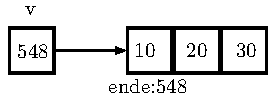
\includegraphics[width=5cm]{ponteiro2.pdf}
        \end{center}
        \vspace{-1em}
        \item Quando passamos um vetor como argumento para uma função, seu conteúdo pode ser alterado
        dentro da função pois estamos passando na realidade o endereço inicial do espaço alocado para o vetor.
    \end{itemize}
    \end{small}
\end{frame}


%%%%%%%%%%%%%%%%%%%%%%%%%%%%%%%%%%%%%%%%%%%%%%
\begin{frame}[fragile]{Ponteiros e Vetores}

    \begin{minted}{c}
        #include <stdio.h>

        void zeraVet(int vet[], int tam) {
            int i;
            for (i = 0; i < tam; i++)
                vet[i] = 0;
        }

        int main() {
            int vetor[] = {1, 2, 3, 4, 5};
            int i;
            zeraVet(vetor, 5);
            for (i = 0; i < 5; i++)
                printf("%d, ", vetor[i]);
            return 0;
        }
    \end{minted}

\end{frame}

%%%%%%%%%%%%%%%%%%%%%%%%%%%%%%%%%%%%%%%%%%%%%%
\begin{frame}[fragile]{Ponteiros e Vetores}

    \begin{itemize}
        \item Tanto é verdade que uma variável vetor possui um endereço, que podemos
        atribuí-la para uma variável ponteiro:
        \begin{minted}{c}
            int a[] = {1, 2, 3, 4, 5};
            int *p;
            p = a;
        \end{minted}

        \item E podemos então usar {\bf p} como se fosse um vetor:
        \begin{minted}{c}
            for (i = 0; i < 5; i++)
                printf("%d\n", p[i]);
        \end{minted}
    \end{itemize}

\end{frame}

%%%%%%%%%%%%%%%%%%%%%%%%%%%%%%%%%%%%%%%%%%%%%%
\begin{frame}[fragile]{Ponteiros e Vetores: Diferenças!}

    \begin{itemize}
        \item Uma variável vetor, diferentemente de um ponteiro, possui um
        endereço fixo.
        \item Isto significa que você não pode tentar atribuir um endereço para
        uma variável do tipo vetor.
    \end{itemize}
    \vspace{-1em}
    \begin{minted}{c}
        #include <stdio.h>
        int main() {
            int a[] = {1, 2, 3, 4, 5};
            int b[5], i;
            b = a;
            for (i = 0; i < 5; i++)
                printf("%d", b[i]);
            return 0;
        }
    \end{minted}

    Ocorre erro de compilação!
\end{frame}

%%%%%%%%%%%%%%%%%%%%%%%%%%%%%%%%%%%%%%%%%%%%%%
\begin{frame}[fragile]{Ponteiros e Vetores: Diferenças!}

    \begin{itemize}
        \item Mas se {\bf b} for declarado como ponteiro não há problemas:
    \end{itemize}
    \vspace{-1em}
    \begin{minted}{c}
        #include <stdio.h>
        int main() {
            int a[] = {1, 2, 3, 4, 5};
            int *b, i;
            b = a;
            for (i = 0 ; i < 5; i++)
                printf("%d, ", b[i]);
            return 0;
        }
    \end{minted}

\end{frame}


%%%%%%%%%%%%%%%%%%%%%%%%%%%%%%%%%%%%%%%%%%%%%%
\begin{frame}[fragile]{Ponteiros e Vetores: Diferenças!}

    O que será impresso pelo programa abaixo?

    \begin{minted}[fontsize=\scriptsize]{c}
        #include <stdio.h>
        int main() {
            int a[] = {1, 2, 3, 4, 5};
            int *b, i;

            b = a;
            printf("Conteudo de b: ");
            for (i = 0; i < 5; i++) {
                printf("%d, ", b[i]);
                b[i] = i*i;
            }
            printf("\nConteudo de a: ");
            for (i = 0; i < 5; i++) {
                printf("%d, ", a[i]);
            }
            printf("\n");
            return 0;
        }
    \end{minted}

\end{frame}


\begin{frame}[fragile]{Extra --- Os argumentos do programa}
    \begin{itemize}
        \item Muitos programas recebem argumentos/parâmetros diretamente na linha de comando
        \begin{itemize}
            \item Exemplos: \texttt{ls -ah}, \texttt{unzip NomeDoArquivo}, \texttt{cp ArqOrigem ArqDestino}, \ldots
        \end{itemize}
        \item Os argumentos de um programa são recebidos como parâmetros da função \cod{main}.
    \end{itemize}
    \begin{minted}[fontsize=\scriptsize]{c}
        int main(int argc, char *argv[]) {
            ...
        }
    \end{minted}
    \begin{itemize}
        \item \textbf{argc} -- \emph{Argument count} -- Número de argumentos do seu programa
        \begin{itemize}
            \item Sempre há pelo menos 1, que é o nome do seu programa
        \end{itemize}
        \item \textbf{argv} -- \emph{Argument values} -- Vetor de
        tamanho \cod{argc} de ponteiros para os argumentos do programa
        (strings)
    \end{itemize}
\end{frame}

\begin{frame}[fragile]{Extra --- Os argumentos do programa --- Exemplo}
    \begin{minted}{c}
        #include <stdio.h>

        int main(int argc, char *argv[]) {
            int i;
            printf("O programa recebeu %d argumentos\n", argc);
            for (i = 0; i < argc; i++)
                printf("\tArgumento %d: %s\n", i, argv[i]);
            return 0;
        }
    \end{minted}
\end{frame}

%%%%%%%%%%%%%%%%%%%%%%%%%%%%%%%%%%%%%%%%%%
%%%%%%%%%%%%%%%%%%%%%%%%%%%%%%%%%%%%%%%%%%
%%%%%%%%%%%%%%%%%%%%%%%%%%%%%%%%%%%%%%%%%%
%%%%%%%%%%%%%%%%%%%%%%%%%%%%%%%%%%%%%%%%%%
%%%%%%%%%%%%%%%%%%%%%%%%%%%%%%%%%%%%%%%%%%
%%%%%%%%%%%%%%%%%%%%%%%%%%%%%%%%%%%%%%%%%%
%%%%%%%%%%%%%%%%%%%%%%%%%%%%%%%%%%%%%%%%%%
%%%%%%%%%%%%%%%%%%%%%%%%%%%%%%%%%%%%%%%%%%
%%%%%%%%%%%%%%%%%%%%%%%%%%%%%%%%%%%%%%%%%%

\section{Exercícios}

%%%%%%%%%%%%%%%%%%%%%%%%%%%%%%%%%%%%%%%%%%%%%%
\begin{frame}[fragile]{\exercicio}
    O que será impresso?
    \vspace{-1em}
    \begin{scriptsize}
        \begin{minted}{c}
            #include <stdio.h>

            int main() {
                int a = 3, b = 2, *p = NULL, *q = NULL;

                p = &a;
                q = p;
                *q = *q + 1;
                q = &b;
                b = b + 1;

                printf("%d\n", *q);
                printf("%d\n", *p);
                return 0;
            }
        \end{minted}
    \end{scriptsize}

\end{frame}

%%%%%%%%%%%%%%%%%%%%%%%%%%%%%%%%%%%%%%%%%%%%%%
\begin{frame}[fragile]{\exercicio}

    Escreva uma função {\bf strcat}
    que recebe como parâmetro 3 strings: {\bf s1}, {\bf s2},  e {\bf sres}.
    A função deve retornar em {\bf sres} a concatenação de {\bf s1} e {\bf s2}.

    Obs: O usuário desta função deve tomar cuidado para declarar {\bf sres} com espaço
    suficiente para armazenar a concatenação de {\bf s1} e {\bf s2}!

\end{frame}


\end{document}
